Os projetos abordados adiante farão uso da IDE Code Composer, baseada em Eclipse, em sua versão 6.1.3 que é a mais recente no momento em que este texto é escrito. oferecida gratuitamente mediante a um cadastro realizado no site da Texas Instruments.

Na hora de instalar a IDE é preciso que sejam marcadas as opções de compatibilidade com a placa em uso, a Tiva C Series TM4C1294 Connected LaunchPad e o MSP432, e ainda seu compilador GCC. Caso contrário, o projeto não poderá ser criado.

Após iniciar o Code Composer, inicie um novo projeto em \textbf{File $>$ New $>$ CCS Project} como mostrado na Figura \ref{fig:novoProjeto01}.

\begin{figure}[H]
	\centering
	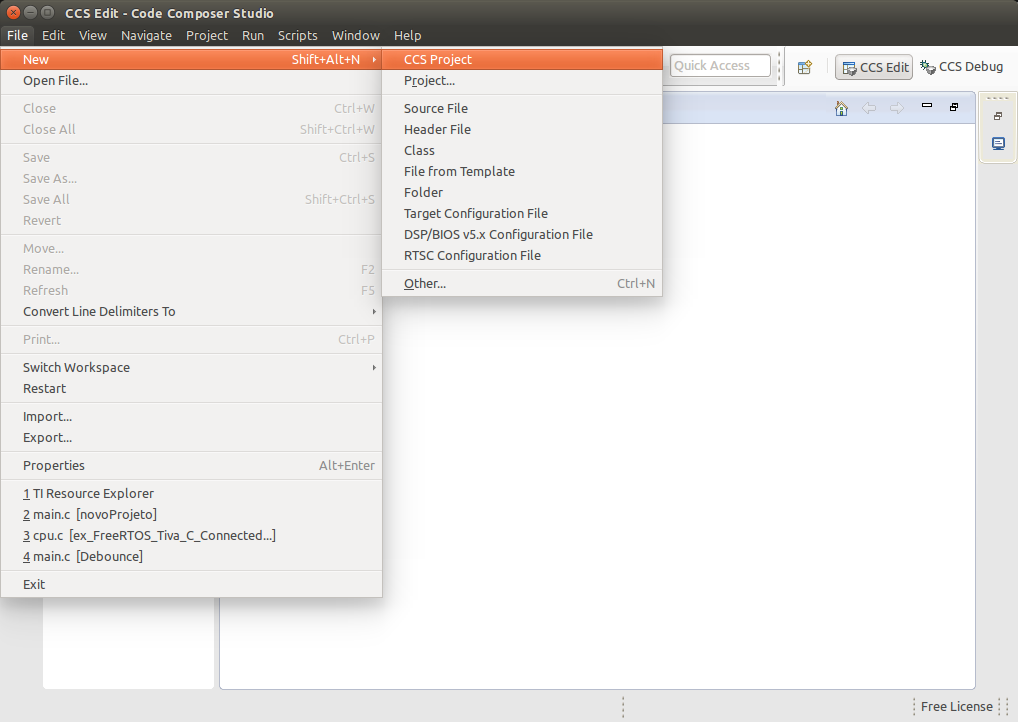
\includegraphics[scale=0.35]{novoProjeto01.png}
	\caption{Criando um novo projeto}
	\label{fig:novoProjeto01}
\end{figure}

Uma janela de configurações será exibida para que o ambiente seja preparado 
para o hardware em uso.

\section{Com o TM4C1294NCPDT}

Em \emph{Target} escolhe-se a opção 
\textbf{Tiva C Series} e no segundo campo \textbf{Tiva TM4C1294NCPDT}, como na Figura \ref{fig:novoProjeto01}.

Em \emph{Connection} será utilizada a \textbf{Stellaris In-Circuit 
Debug Interface} para a programação e debug do microcontrolador.

Após isso, escolhe-se um nome para o projeto e o diretório que será armazenado, 
que é normalmente o local do workspace padrão marcando a opção \textbf{Use 
default location}.

A Texas Instruments disponibiliza um compilador próprio porém será usado aqui o 
GCC, compilador de código aberto sob a licença GNU. Portanto, em \emph{Compile 
version} escolhe-se a opção \textbf{GNU} com a versão mais recente.
As outras opções não precisam ser alteradas.

\begin{figure}[H]
	\centering
	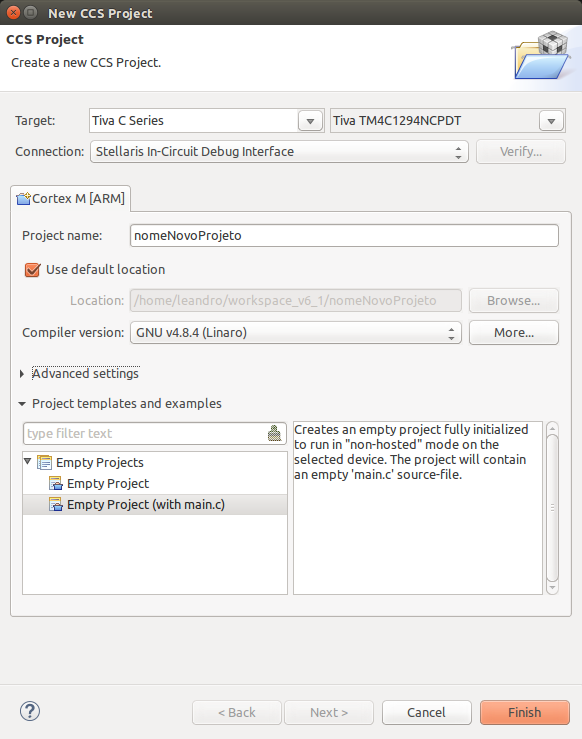
\includegraphics[scale=0.5]{novoProjeto02.png}
	\caption{Configurando o projeto}
	\label{fig:novoProjeto02}
\end{figure}

Clicando em \emph{Finish} o projeto será criado. Para o correto funcionamento 
do compilador GCC devem-se ainda ser feitos mais alguns ajustes.

Selecionando o projeto criado na barra lateral \emph{Project Explorer}, vá em 
\textbf{Project $>$ Properties} como na Figura \ref{fig:novoProjeto03}.

\begin{figure}[H]
	\centering
	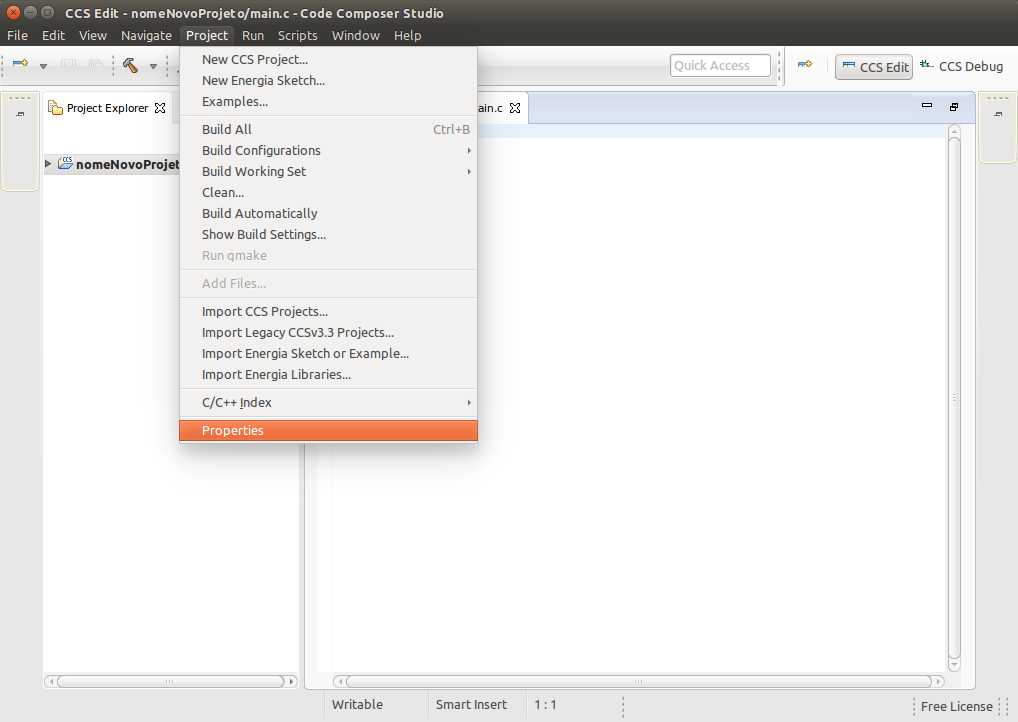
\includegraphics[scale=0.35]{novoProjeto03.png}
	\caption{Abrindo propriedades do projeto}
	\label{fig:novoProjeto03}
\end{figure}

Na janela de propriedades selecione \textbf{Build $>$ GNU Compiler $>$ 
Symbols}. Adicione um novo símbolo clicando no botão \emph{Add} como na Figura 
\ref{fig:novoProjeto04}. Na janela que se abre digite 
\textbf{TARGET\_IS\_TM4C129\_RA1} e clique em \emph{OK}. Adicione ainda o 
símbolo \textbf{gcc}. Esses símbolos não podem conter erros de escrita, caso 
contrário causarão erros na hora da compilação. Ao se ter os três símbolos 
mostrados na Figura \ref{fig:novoProjeto04}, selecione \textbf{Build $>$ GNU 
Linker $>$ Basic}. Na opção \emph{Set start address} digite \textbf{\_start} 
como na Figura \ref{fig:novoProjeto05} e clique em \emph{OK}.

\begin{figure}[H]
	\centering
	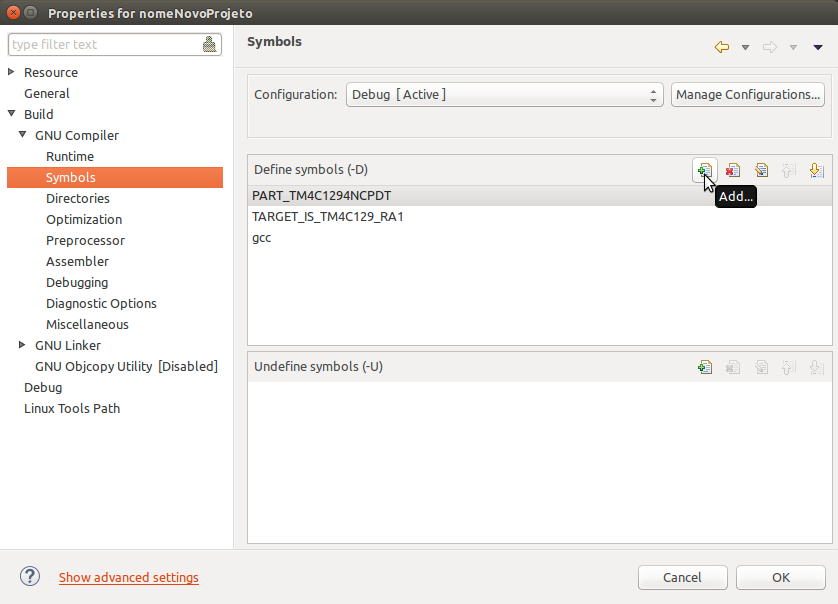
\includegraphics[scale=0.4]{novoProjeto04.png}
	\caption{Adicionando símbolo para a compilação no GCC}
	\label{fig:novoProjeto04}
\end{figure}

\begin{figure}[H]
	\centering
	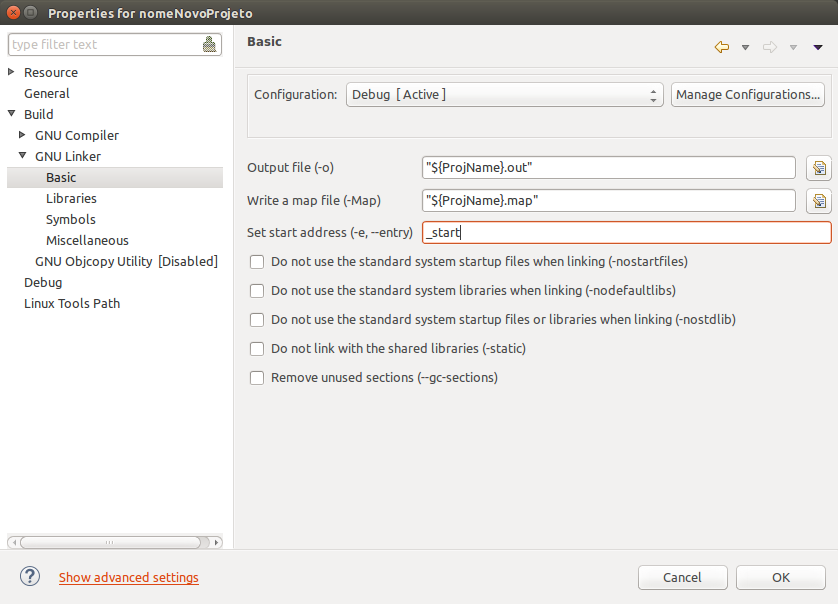
\includegraphics[scale=0.4]{novoProjeto05.png}
	\caption{Configurando endereço de início do Linker do GCC}
	\label{fig:novoProjeto05}
\end{figure}

Ao fim desses passos o projeto estará criado e poderá ser compilado no Code Composer utilizando o GCC.

\section{Com o MSP432P401R}

Em \emph{Target} escolhe-se a opção \textbf{MSP432 Family} e no segundo campo \textbf{MSP432P401R}.

Em \emph{Connection} será utilizada a \textbf{Texas Instruments XDS110 USB Debug Probe} para a programação e debug do microcontrolador.

Após isso, escolhe-se um nome para o projeto e o diretório que será armazenado, 
que é normalmente o local do workspace padrão marcando a opção \textbf{Use 
default location}.

Novamente, em \emph{Compile 
version} escolhe-se a opção \textbf{GNU} com a versão mais recente, para utilizar o GCC como compilador.
As outras opções não precisam ser alteradas.

\begin{figure}[H]
	\centering
	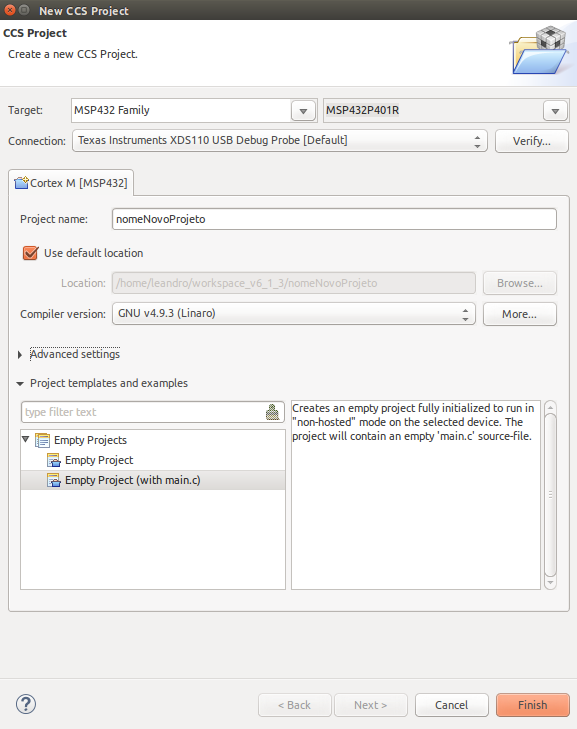
\includegraphics[scale=0.5]{novoProjeto06.png}
	\caption{Configurando o projeto}
	\label{fig:novoProjeto06}
\end{figure}

Para o MSP432 não é necessária nenhuma alteração nas propriedades do arquivo, utilizando o GCC. Após criar o projeto já pode-se iniciar a implementação.